\documentclass[a4paper,UTF8]{article}
\usepackage{ctex}
\usepackage[margin=1.25in]{geometry}
\usepackage{color}
\usepackage{graphicx}
\usepackage{amssymb}
\usepackage{amsmath}
\usepackage{amsthm}
%\usepackage[thmmarks, amsmath, thref]{ntheorem}
\theoremstyle{definition}
\newtheorem*{solution}{Solution}
\newtheorem*{prove}{Proof}
\usepackage{multirow}
\usepackage{url}
\usepackage{enumerate}
\usepackage{algorithm}
\usepackage{algorithmic}
\renewcommand{\algorithmicrequire}{\textbf{Input:}}
\renewcommand{\algorithmicensure}{\textbf{Procedure:}}
\renewcommand\refname{参考文献}
% \usepackage{caption}
% \usepackage{subfigure}

%--

%--
\begin{document}
\title{实验3. 强化学习实践}
\author{MF1733034, 李青坪, \url{lqp19940918@163.com}}
\maketitle

\section*{综述}
与传统的监督、无监督学习不同,强化学习的过程需要与学习环境进行交互,利用环境反馈信息进行学习。
因此在本次实验中,我们将脱离从训练数据集中获取学习模型的学习框架,转向与动态的学习环境打交道。
本次实验,我们将从学习环境的安装、常用强化学习 算法的实现,强化学习算法改进这些方面完整的体会一次强化学习研究的过程。

本次实验采用的强化学习环境为OpenAI开源的Gym。Gym中集成了很多强化学习的实验环境,并为测试强化学习提供了很多学习任务,
如CartPole和MountainCar等。在DQN算法实现中会用到深度学习工具,本次实验采用PyTorch,PyTorch提供了神经网络的搭建模型,
方便我们实现DQN算法。

\section*{实验二. }
Gym为我们提供了一些基础学习任务,但是在这些任务里面,状态空间都是连续的,而Q-learning算法的状态空间是离散的。
所以本次实验的首要任务就是对状态空间离散化,通过Gym文档中提供的状态-动作空间的查询命令,
我们知道CartPole、MountainCar和Acrobot三个任务的状态-动作空间分别为(4, 2), (2, 3), (6, 3),我们需要对这些空间进行离散化。
本次实验采用的方法是将连续的空间分成等间隔的n份(n为每个维度上划分的块数)。具体算法如下:

	设observation[i]表示第i维状态观测值,$STATE\_THRESHOLD[i]$表示第i维状态的下界,$bound\_width$表示第i维状态的观测值的数据宽度,
$STATE\_NUM[i]$表示自定义的第i维状态的离散状态数目。
则对于每一个观测值,求出其在离散化的状态空间中对应的下标即可。
\begin{align*}
	&state\_index = \\
	&(observation[i] - STATE\_THRESHOLD[i])/bound\_width * STATE\_NUM[i]
\end{align*}
通过状态空间离散化,即将连续的观测空间状态转换到离散的空间上来,我们即可使用Q-learning算法进行强化学习。

Q-learning算法实现的思路如下:
\begin{itemize}
	\item 首先初始化一张Q(s, a)表,里面的每一行表示在状态s,执行动作a所拥有的价值。
	\item 对每一个片段执行以下操作:
	\item 初始化状态s
	\item 对每一个片段里的每一个步骤执行以下操作:
	\item 在状态s使用$\epsilon$ 贪心策略选出动作a
	\item 执行动作a,得到奖励r和下一个状态$s^`$
	\item 更新Q值:$Q(s, a) \gets Q(s, a) + \alpha [r + \gamma max_{a^`}Q(s^`, a^`) - Q(s, a)]$
	\item $s \gets s^`$
\end{itemize}

算法实现思路比较简单,而且代码也不是特别复杂,想要实验可以成功的完成任务,最重要的还是参数的调整。在本次实验中,
探索率$\epsilon$初始设置为1.0,最小值设置为0.01,按照指数级别递减;学习率$\alpha$初始设置为0.5,最小值设置为0.1,按照指数级别递减;
衰减值$\gamma$设置为0.99恒定不变。

针对CartPole任务,最大观测长度设置为20000,片段数设置为1000(考虑到接近收敛的时候,基本都能保证杆子不倒下来,故设置在连续200次成功解决CartPole问题后就
认为已经收敛,则终止片段循环),成功解决CartPole问题的步骤数设置为199。每个状态维度的可操作状态数设置为(1, 1, 6, 5),表示只考虑杆子的角度和角速度,
忽略小车的位置和速度。虽然损失两个状态,但对解决CartPole问题不会产生影响。

针对MountainCar任务,最大观测长度设置为2000,片段数设置为1000(考虑到接近收敛的时候,基本都能保证小车到达旗杆处,故设置在连续200次成功解决MountainCar问题后就
认为已经收敛,则终止片段循环)。每个状态维度的可操作状态数设置为(8, 8),表示小车的位置和速度各有8个可操作状态。

针对Acrobot任务,最大观测长度设置为2000,片段数设置为1000(考虑到接近收敛的时候,基本都能保证关节达到系统设定的高点,故设置在连续200次成功解决Acrobot问题后就
认为已经收敛,则终止片段循环)。每个状态维度的可操作状态数设置为(1, 1, 1, 1, 10, 10),表示只考虑两个杆子的角速度,
忽略它们的角度。虽然损失两个状态,但对解决Acrobot问题不会产生影响。

对三个强化学习任务分别进行5次实验,得到多条轨迹上reward的均值和标准差:
\leftline{CartPole:}

	\begin{tabular}{|c|c|c|c|c|c|}
	
		\hline
		
		\hline
		
		- & 1 & 2 & 3 & 4 & 5 \\
		
		\hline
		
		均值 & 7111.80 & 7376.67 & 7636.14 & 7219.83 & 7426.34\\

		\hline

		标准差 & 6009.24 & 5946.63 & 6190.02 & 6025.62 & 6020.15\\
		
		\hline
	
	\end{tabular}
	
\leftline{MountainCar:}

	\begin{tabular}{|c|c|c|c|c|c|}
	
		\hline
		
		\hline
		
		- & 1 & 2 & 3 & 4 & 5 \\
		
		\hline
		
		均值 & -163.78 & -178.46 & -185.27 & -161.381 & -212.69\\

		\hline

		标准差 & 22.57 & 129.53 & 7.98 & 276.15 & 32.82\\
		
		\hline
	
	\end{tabular}
	
\leftline{Acrobot:}

	\begin{tabular}{|c|c|c|c|c|c|}
	
		\hline
		
		\hline
		
		- & 1 & 2 & 3 & 4 & 5 \\
		
		\hline
		
		均值 & -144.01 & -103.94 & -105.65 & -88.99 & -261.28\\

		\hline

		标准差 & 29.49 & 193.17 & 122.38 & 63.22 & 271.97\\
		
		\hline
	
	\end{tabular}

\section*{实验三. }
由于 Q-learning 需要穷举状态-动作对,所以面对连续状态-动作空间, Q-learning 无法适用。但是值函数近似 Q-learning 方法能够解决此类问题。
若将值函数近似模型选取为一个深度网络,即为 Deep Q-learning (DQN) 算法。DQN 算法基于 Q-learning,算法框架和 Q-learning 完全相同,不同之处在于 Q 函数 的表示和更新方式上。
DQN 中 Q 函数用一个深度网络表示,记为 Q(s, a; $\theta$),其中 s 表示 状态,a 表示执行的动作,$\theta$ 表示网络参数。DQN 的目的是得到一个 Q 函数网络,对于一 组状态动作对 (s, a),
使得 Q 函数网络的输出 Q(s, a; $\theta$) 等于 (s, a) 下真实的 Q 值。具体到 深度网络表示的 Q 函数模型上,
Q 函数的学习问题转化为了如何学习一组深度网络参数 $\theta$ 使网络输出近似于真实的 Q 值。
	
本次实验中,我们采用PyTorch提供的神经网络模型建立我们所需的Q-evaluation网络,输入层神经元数目为可观测的状态数目;
隐藏层有一层,这里设置隐藏层有$hidden\_num$个神经元($hidden\_num$由具体的任务指定,如CartPole的$hidden\_num$设为50);输出层的神经元个数为动作的数目。
新建一个DQN类,表示我们将要实现的算法,私有属性memory表示大小为N的重现内存,
这里设置N=2000,设置损失函数为PyTorch提供的nn.MSELoss()函数,即平方损失函数,公式如下:
$$loss(x, y) = \frac{1}{N} \sum_{i=1}^N |x - y|^2$$
使用torch.optim.Adam()作为学习的优化器,它利用梯度的一阶矩估计和二阶矩估计动态调整每个参数的学习率,
参数为Q-evaluation网络,学习率$\alpha$的初始值设为0.008;
探索率$\epsilon$初始设置为1,最小值设置为0.01,随片段episode的增加呈指数级别减小;衰减值$\gamma$设置为0.99恒定不变;
算法中每次从memory中抽取的MINI\_BATCH数目为32。

DQN算法实现思路如下:
\begin{itemize}
	\item 初始化大小为(N x (状态数+2))的memory矩阵。
	\item 新建Q-target网络和Q-evaluation网络,即完成状态动作函数的初始化。
	\item 对每一个片段执行以下操作:
	\item 初始化状态s
	\item 对每一个片段里的每一个步骤执行以下操作:
	\item 在状态s使用$\epsilon$ 贪心策略选出动作$a_t$
	\item 执行动作$a_t$,得到奖励$r_t$和下一个状态$s_{t+1}$
	\item 将($s_t$, $a_t$, $r_t$, $s_{t+1}$)存入memory中
	\item 从memory中随机抽取MINI\_BATCH个数据
	\item 对抽取到的每个数据计算$y_i = r_j + \gamma max_{a^`} Q(s_{t+1}, a^`; \theta)$
	\item 将$y_j$和$Q(s_j, a; \theta)$带入损失函数,修正$\theta$
\end{itemize}

针对CartPole任务,最大观测长度设置为20000,片段数设置为200(实验发现,在执行200次片段过后就接近收敛)。输入层神经元个数为4,表示4个可观测状态;
隐藏层神经元个数为50;输出层神经元个数为2。同时,需要修改reward的值,使状态动作函数尽快收敛,修改思路如下:
考虑小车的位置离中点越近reward值越高、杆子越保持垂直reward值越高。

针对MountainCar任务,最大观测长度设置为2000,片段数设置为400(考虑到接近收敛的时候,基本都能保证小车到达旗杆处,故设置在连续300次成功解决MountainCar问题后就
认为已经收敛,则终止片段循环)。输入层神经元个数为2,表示2个可观测状态;隐藏层神经元个数为25;输出层神经元个数为3。
修改reward值:小车离坡道最低点越远reward值越高、一旦小车达到最高点则给一个较大的reward。

针对Acrobot任务,最大观测长度设置为2000,片段数设置为300。输入层神经元个数为6,表示6个可观测状态;
隐藏层神经元个数为50;输出层神经元个数为2。该任务没有修改reward值,利用系统给定的reward值就能很好的完成强化学习。

网络训练误差随训练轮数的变化关系:
\begin{figure}
	\centering                                                          %居中                  %第一张子图
	\begin{minipage}{7cm}
		\centering                                                          %子图居中
		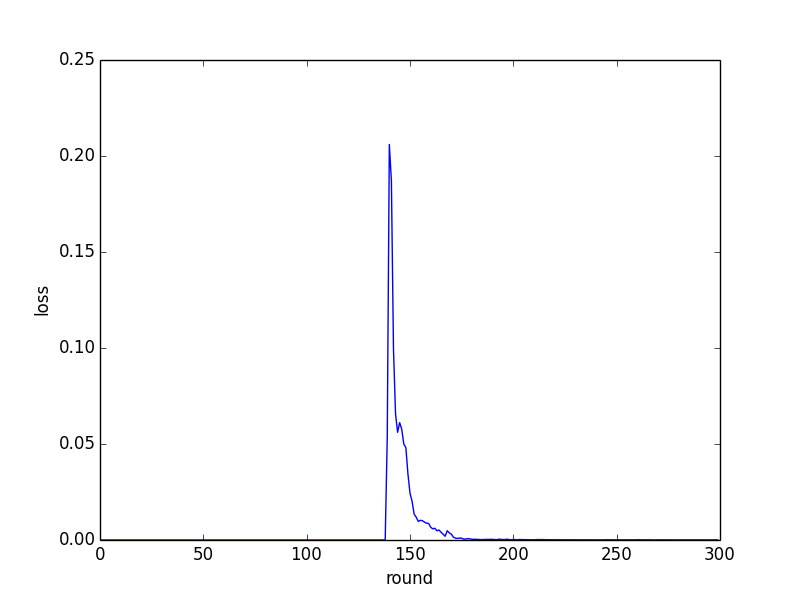
\includegraphics[scale=0.5]{exper4_cartpole_loss1.png}               %以pic.jpg的0.5倍大小输出
	\end{minipage}
				%第二张子图
	\begin{minipage}{7cm}
		\centering                                                          %子图居中
		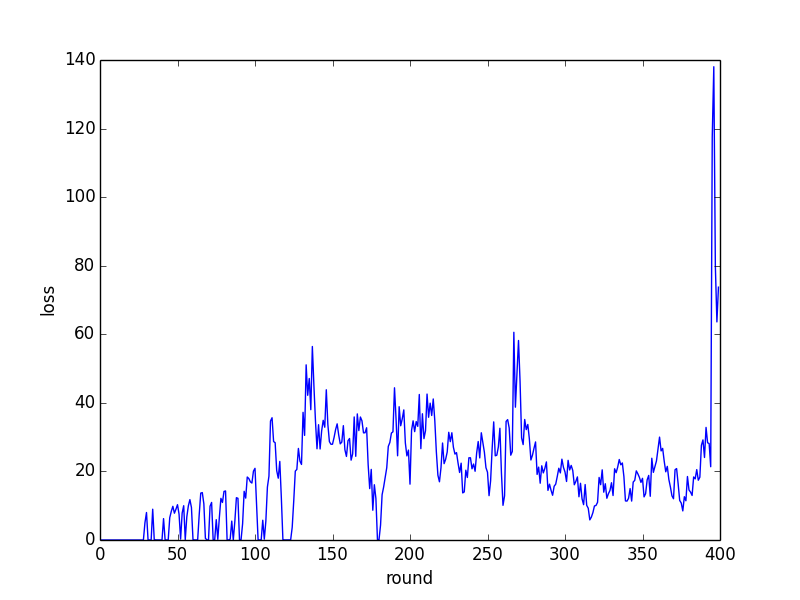
\includegraphics[scale=0.4]{exper4_mountaincar_loss.png}                %以pic.jpg的0.5倍大小输出
	\end{minipage}

	\begin{minipage}{7cm}
		\centering                                                          %子图居中
		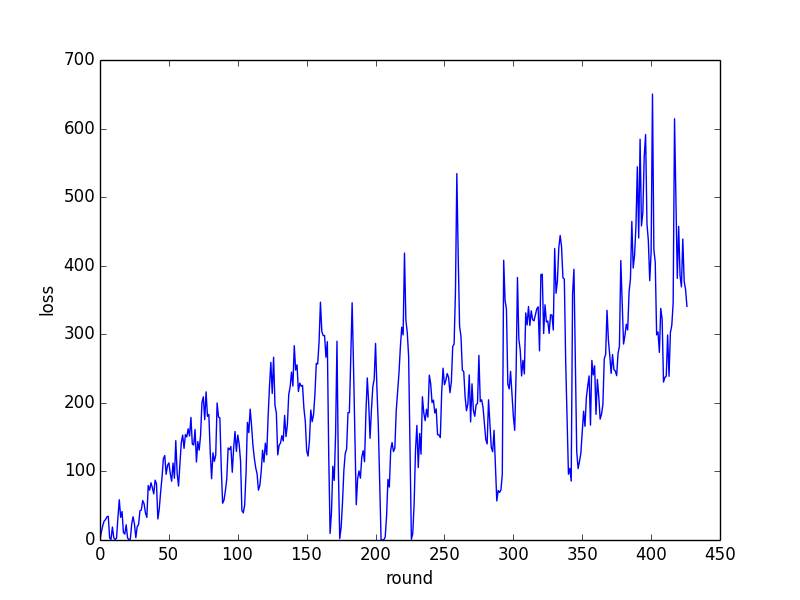
\includegraphics[scale=0.4]{exper4_acrobot_loss.png}                %以pic.jpg的0.5倍大小输出
	\end{minipage}}
	\caption{loss比较} %                         %大图名称
	\label{fig:1} 
\end{figure}

对三个强化学习任务分别进行5次实验,得到多条轨迹上reward的均值和标准差:
\leftline{CartPole:}

	\begin{tabular}{|c|c|c|c|c|c|}
	
		\hline
		
		\hline
		
		- & 1 & 2 & 3 & 4 & 5 \\
		
		\hline
		
		均值 & 19667.55 & 19575.45 & 19489.12 & 19456.23 & 19535.27\\

		\hline

		标准差 & 1953.69 & 2357.74 & 2471.89 & 2001.16 & 1959.57\\
		
		\hline
	
	\end{tabular}
	
\leftline{MountainCar:}

	\begin{tabular}{|c|c|c|c|c|c|}
	
		\hline
		
		\hline
		
		- & 1 & 2 & 3 & 4 & 5 \\
		
		\hline
		
		均值 & -135.28 & -134.68 & -147.42 & -133.76 & -145.34\\

		\hline

		标准差 & 34.46 & 36.66 & 26.81 & 33.58 & 65.38\\
		
		\hline
	
	\end{tabular}
	
\leftline{Acrobot:}

	\begin{tabular}{|c|c|c|c|c|c|}
	
		\hline
		
		\hline
		
		- & 1 & 2 & 3 & 4 & 5 \\
		
		\hline
		
		均值 & -112.25 & -103.86 & -103.35 & -108.71 & -151.89\\

		\hline

		标准差 & 42.20 & 33.14 & 42.01 & 49.26 & 129.11\\
		
		\hline
	
	\end{tabular}

\section*{实验四. }
由于 Q-learning 需要穷举状态-动作对,所以面对连续状态-动作空间, Q-learning 无法适用。但是值函数近似 Q-learning 方法能够解决此类问题。
若将值函数近似模型选取为一个深度网络,即为 Deep Q-learning (DQN) 算法。DQN 算法基于 Q-learning,算法框架和 Q-learning 完全相同,不同之处在于 Q 函数 的表示和更新方式上。
DQN 中 Q 函数用一个深度网络表示,记为 Q(s, a; $\theta$),其中 s 表示 状态,a 表示执行的动作,$\theta$ 表示网络参数。DQN 的目的是得到一个 Q 函数网络,对于一 组状态动作对 (s, a),
使得 Q 函数网络的输出 Q(s, a; $\theta$) 等于 (s, a) 下真实的 Q 值。具体到 深度网络表示的 Q 函数模型上,
Q 函数的学习问题转化为了如何学习一组深度网络参数 $\theta$ 使网络输出近似于真实的 Q 值。
	
本次实验中,我们采用PyTorch提供的神经网络模型建立我们所需的Q-target网络和Q-evaluation网络,输入层神经元数目为可观测的状态数目;
隐藏层有一层,这里设置隐藏层有$hidden\_num$个神经元($hidden\_num$由具体的任务指定,如CartPole的$hidden\_num$设为50);输出层的神经元个数为动作的数目。
新建一个DQN类,表示我们将要实现的算法,私有属性memory表示大小为N的重现内存,
这里设置N=2000,设置损失函数为PyTorch提供的nn.MSELoss()函数,即平方损失函数,公式如下:
$$loss(x, y) = \frac{1}{N} \sum_{i=1}^N |x - y|^2$$
使用torch.optim.Adam()作为学习的优化器,它利用梯度的一阶矩估计和二阶矩估计动态调整每个参数的学习率,
参数为Q-evaluation网络,学习率$\alpha$的初始值设为0.008;
探索率$\epsilon$初始设置为1,最小值设置为0.01,随片段episode的增加呈指数级别减小;衰减值$\gamma$设置为0.99恒定不变;
Q-target更新频率设置为每学习100次更新一次;算法中每次从memory中抽取的MINI\_BATCH数目为32。

DQN算法实现思路如下:
\begin{itemize}
	\item 初始化大小为(N x (状态数+2))的memory矩阵。
	\item 新建Q-target网络和Q-evaluation网络,即完成状态动作函数的初始化。
	\item 对每一个片段执行以下操作:
	\item 初始化状态s
	\item 对每一个片段里的每一个步骤执行以下操作:
	\item 在状态s使用$\epsilon$ 贪心策略选出动作$a_t$
	\item 执行动作$a_t$,得到奖励$r_t$和下一个状态$s_{t+1}$
	\item 将($s_t$, $a_t$, $r_t$, $s_{t+1}$)存入memory中
	\item 从memory中随机抽取MINI\_BATCH个数据
	\item 对抽取到的每个数据计算$y_i = r_j + \gamma max_{a^`} Q(s_{t+1}, a^`; \theta)$
	\item 将$y_j$和$Q(s_j, a; \theta)$带入损失函数,修正$\theta$
\end{itemize}

针对CartPole任务,最大观测长度设置为20000,片段数设置为200(实验发现,在执行200次片段过后就接近收敛)。输入层神经元个数为4,表示4个可观测状态;
隐藏层神经元个数为50;输出层神经元个数为2。同时,需要修改reward的值,使状态动作函数尽快收敛,修改思路如下:
考虑小车的位置离中点越近reward值越高、杆子越保持垂直reward值越高。

针对MountainCar任务,最大观测长度设置为2000,片段数设置为400(考虑到接近收敛的时候,基本都能保证小车到达旗杆处,故设置在连续300次成功解决MountainCar问题后就
认为已经收敛,则终止片段循环)。输入层神经元个数为2,表示2个可观测状态;隐藏层神经元个数为25;输出层神经元个数为3。
修改reward值:小车离坡道最低点越远reward值越高、一旦小车达到最高点则给一个较大的reward。

针对Acrobot任务,最大观测长度设置为2000,片段数设置为300。输入层神经元个数为6,表示6个可观测状态;
隐藏层神经元个数为50;输出层神经元个数为2。该任务没有修改reward值,利用系统给定的reward值就能很好的完成强化学习。

网络训练误差随训练轮数的变化关系:
\begin{figure}
	\centering                                                          %居中
                  %第一张子图
	\begin{minipage}{7cm}\centering                                                          %子图居中
	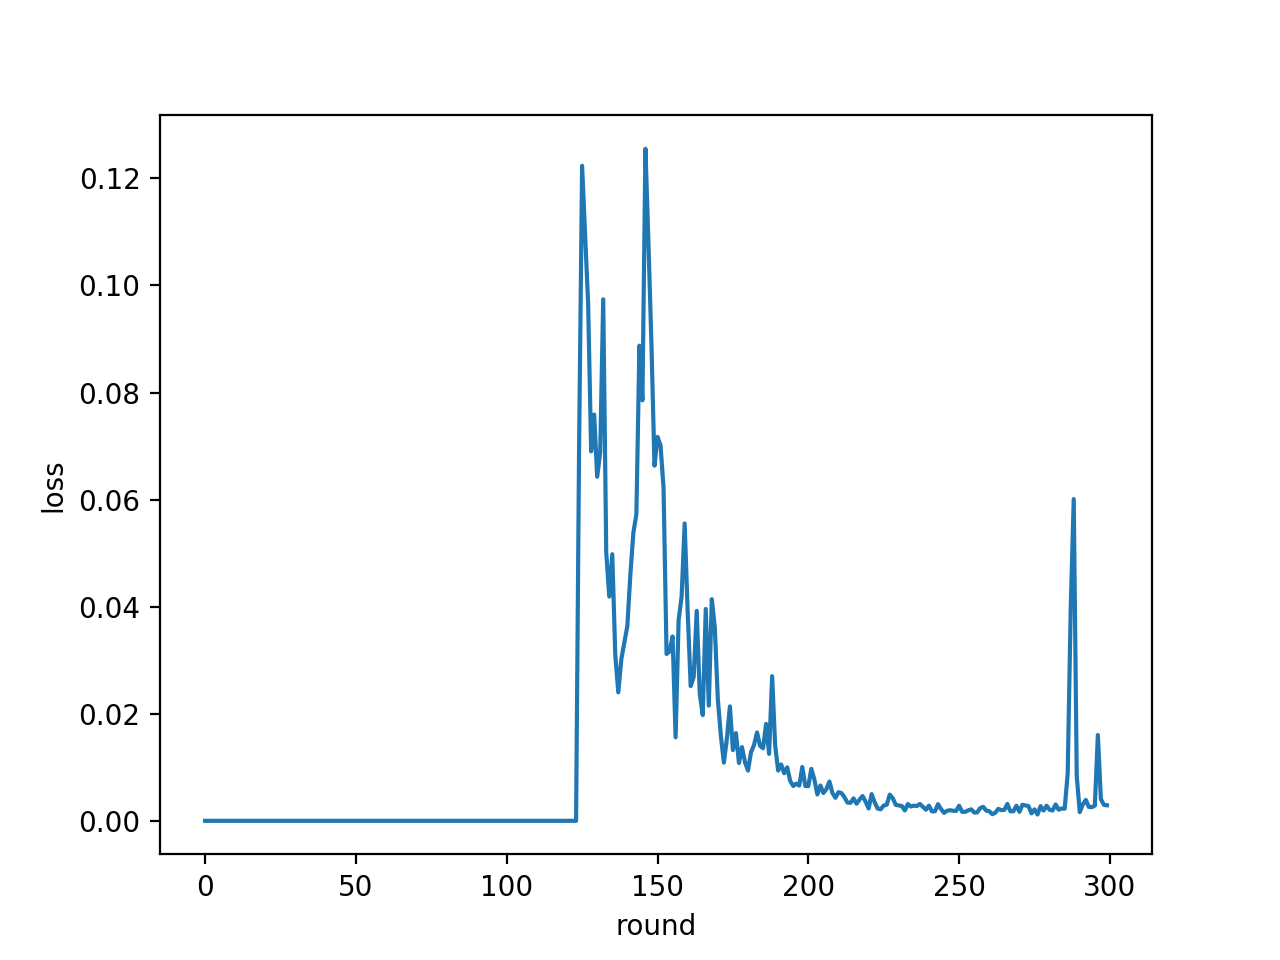
\includegraphics[scale=0.5]{exper3_cartpole_loss.png}               %以pic.jpg的0.5倍大小输出
	\end{minipage}
				%第二张子图
	\begin{minipage}{7cm}
		\centering                                                          %子图居中
		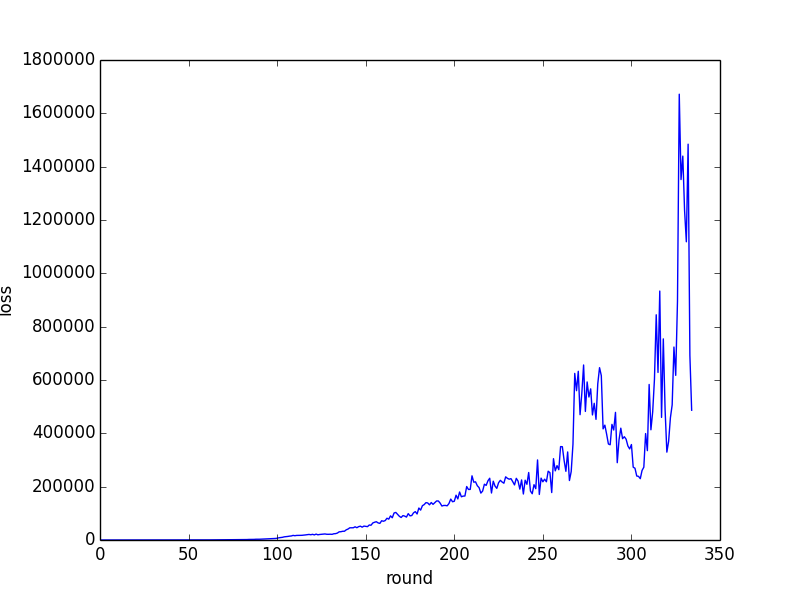
\includegraphics[scale=0.4]{exper3_mountaincar_loss.png}                %以pic.jpg的0.5倍大小输出
	\end{minipage}

	\begin{minipage}{7cm}
		\centering                                                          %子图居中
		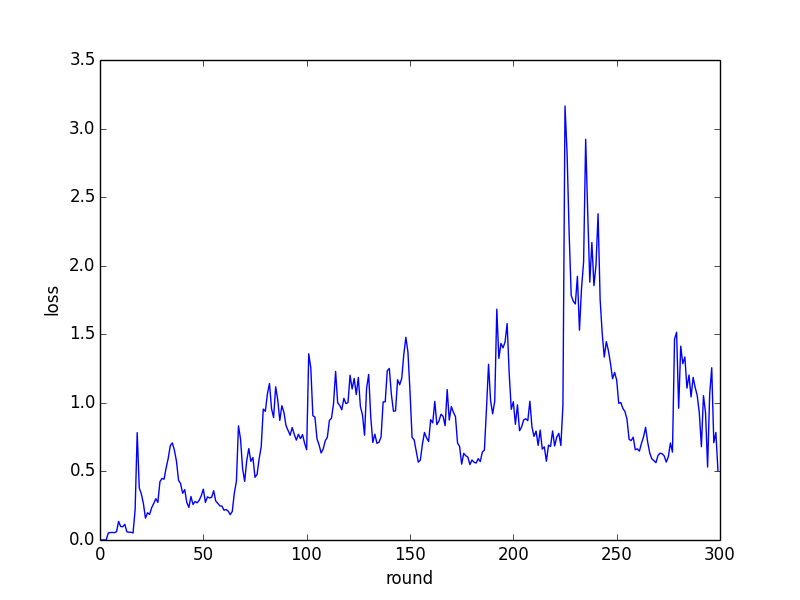
\includegraphics[scale=0.4]{exper3_acrobot_loss.png}                %以pic.jpg的0.5倍大小输出
	\end{minipage}}

	\caption{name of the figure} %                         %大图名称
	\label{fig:2} 
\end{figure}

对三个强化学习任务分别进行5次实验,得到多条轨迹上reward的均值和标准差:
\leftline{CartPole:}

	\begin{tabular}{|c|c|c|c|c|c|}
	
		\hline
		
		\hline
		
		- & 1 & 2 & 3 & 4 & 5 \\
		
		\hline
		
		均值 & 19667.55 & 19575.45 & 19489.12 & 19456.23 & 19535.27\\

		\hline

		标准差 & 1953.69 & 2357.74 & 2471.89 & 2001.16 & 1959.57\\
		
		\hline
	
	\end{tabular}
	
\leftline{MountainCar:}

	\begin{tabular}{|c|c|c|c|c|c|}
	
		\hline
		
		\hline
		
		- & 1 & 2 & 3 & 4 & 5 \\
		
		\hline
		
		均值 & -135.28 & -134.68 & -147.42 & -133.76 & -145.34\\

		\hline

		标准差 & 34.46 & 36.66 & 26.81 & 33.58 & 65.38\\
		
		\hline
	
	\end{tabular}
	
\leftline{Acrobot:}

	\begin{tabular}{|c|c|c|c|c|c|}
	
		\hline
		
		\hline
		
		- & 1 & 2 & 3 & 4 & 5 \\
		
		\hline
		
		均值 & -112.25 & -103.86 & -103.35 & -108.71 & -151.89\\

		\hline

		标准差 & 42.20 & 33.14 & 42.01 & 49.26 & 129.11\\
		
		\hline
	
	\end{tabular}

\end{document}